\chapter{La linguistique ça vous parle ?}\label{chap:linguistic}

La \gls{phon}, normalement maintenant, vous savez à peu près ce que
c'est. Mais qu'en est-il de la \gls{linguistic} ?

Ben il se retrouve que la \gls{phon} en est une de ses branches.

\begin{center}
    \begin{figure}[h]
      \centering
        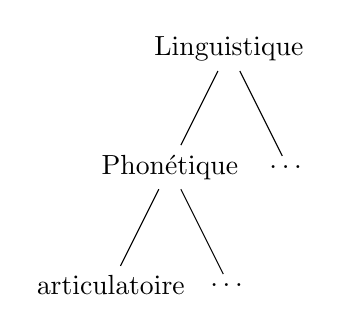
\begin{tikzpicture}
          \node {Linguistique}
          child { node {Phonétique}  
            child { node { articulatoire } }
            child { node { \dots } }
          }
          child { node {\dots} } 
          ;
        \end{tikzpicture}
    \caption{Branches de la \gls{linguistic}}
    \label{fig:branch-phon}
  \end{figure}
\end{center}
Cela vous paraît peut être surprenant que je m'amuse à remonter les
branches. Pourtant c'est une démarche assez naturelle. On a
fondamentalement deux façons d'étudier un domaine.

\begin{enumerate}
\item La première consiste à partir du général  pour aller vers le
  particulier.
\item La seconde consiste à faire l'inverse.  
\end{enumerate}

 L'objet de ce livre étant de traiter de la \gls{phon} anglaise il m'a
 paru plus opportun de démarrer avec une vue d'ensemble de la
 \gls{phon}. Mais il me semble tout de même nécessaire de dessiner le
 contour de ce qu'est la \gls{linguistic} qui, hélas, n'est pas une
 science très connue du grand public alors qu'elle est probablement la
 plus fondamentale.

 Au commencement était le verbe\footnote{Il est amusant de voir qu'en
   anglais ce n'est pas tout à fait pareil \exEN{In the beginning was
     the Word} qui se traduit littéralement par \exFR{Au commencement
     il y avait le Mot}.} aurait dit l'autre, et ce n'est pas pour
 rien, le langage oral est ce que nous partageons tous nous autres
 êtres humains. Quelle que soit votre activité, dans tous les cas vous
 communiquez par le langage.

 \'Etrangement à l'école nous ne l'étudions pas beaucoup ce
 langage. Lors des petites classes on nous fait apprendre les règles
 par c{\oe}ur puis on passe vite à la littérature (dès le collège) ou
 à la philosophie (au lycée). Il en va de même pour les langues
 étrangères. Pourtant lorsqu'on y réfléchi c'est tout de même étrange
 de se dire que nous partageons tous la même faculté de produire du
 langage mais que l'endroit où nous naissons va considérablement
 affecter les règles que nous allons utiliser pour le produire.

 Bref, sans plus attendre, laissons la parole aux professionnels que sont
 messieurs \textsc{Paul Burleigh} et \textsc{Peter Skandera} avec leur
 livre~\cite{burleigh} qui était à la base destiné à un public de langue allemande.

\newpage
\minitoc
\newpage

\section{Prescriptivisme et descriptivisme}

Le débat entre prescriptivistes et descriptivistes est un éternel
débat dont j'avais déjà parlé dans cet
\href{http://doyouspeakenglish.fr/prescriptiviste-ou-descriptiviste/}{article}
de
blog\footnote{\url{http://doyouspeakenglish.fr/prescriptiviste-ou-descriptiviste/}}. Malheureusement
en France nous n'avons pas vraiment le droit de nous exprimer
puisqu'il existe une institution qui décide pour tout le monde des
règles de la langue française. Du coup, cela pourra paraître, au
premier abord, être une querelle de spécialiste. Mais il n'en est
rien, et ce serait une erreur de prendre ça à la légère ! C'est une
véritable question de fond !

\begin{center}
\begin{mdframed}[style=citestyle, frametitle={Extrait de~\cite{Burleigh}}]
  \exEN{``From ancient times until the present, language purists have
    believed that the task of the grammarian is to \emph{prescribe}
    (rather than \emph{describe}) correct usage that all educated
    people should use in speaking and
    writing. \textbf{Prescriptive} language scholars have
    laid down rules that are often based on Latin and Greek, on a
    classical canon of literary works, on the origin of particular
    words, on logic, or simply on their personal likes and
    dislikes. Prescriptivists have been criticised for not taking
    sufficient account of ongoing language change and stylistic
    variation. By contrast, the aim of linguistics is to
    \emph{describe} language objectively and
    systematically. \textbf{Descriptive} linguists observe
    and analyse language as it is used naturally in any given speech
    community [\emph{\textgerman{Sprachgemeinschaft}}], and they
    attempt to discover the rules and regularities of the underlying
    language system, or code.''}
\end{mdframed}  
\end{center}

Dès la première ligne on observe à quel point la question est
ancienne. Il est amusant de remarquer que le mot prescriptiviste a la
même racine que le verbe prescrire qui est utilisé par le médecin
lorsque nous sommes malades. Cela voudrait-il dire que certaines
personnes penseraient que d'autres sont malades de la langue ?

Occupons-nous désormais de la traduction.

\begin{center}
\begin{mdframed}[style=tradstyle, frametitle={\exFR{Traduction} de l'extrait précédent}]
  \exFR{Depuis les temps anciens jusqu'à nos jours, les puristes de la
    langue croyaient que la tâche du grammairien est de \emph{prescrire}
(plutôt que \emph{décrire}) l'usage correct que tous les gens éduqués
devraient utiliser pour parler et écrire. Les professeurs de langues
\textbf{prescriptifs} ont établi des règles qui sont souvent
basées sur le latin et le grec, sur des canons classiques d'{\oe}uvres
littéraires, sur l'origine de certains mots, sur la logique, ou simplement sur
leurs goûts personnels en fonction de ce qu'ils aiment et n'aiment
pas. Les prescriptivistes ont été critiqués pour ne pas tenir compte
suffisamment du changement de la langue en usage et des variations
stylistiques. En revanche, le but de la linguistique est de
\emph{décrire} le langage objectivement et systématiquement. Les
linguistes \textbf{descriptivistes} observent et analysent
le langage tel qu'il est utilisé naturellement dans n'importe quel
discours donné dans une communauté
[\textgerman{\emph{Sprachgemeinschaft}}], et ils tentent de découvrir
les  règles et les régularités du système de langue sous-jacent, ou
code.}
\end{mdframed}  
\end{center}


Pour la faire simple on va dire que les prescriptivistes sont les
conservateurs et les descriptivistes les progressistes. Alors vu de
France c'est un peu compliqué parce que nous sommes fondamentalement
dans un pays prescriptiviste puisque une vieille bande d'illuminés
qui se prétendent immortels ont un droit absolu sur la façon de dicter
les lois de la langue française.

Bien heureusement, en France comme dans tous les pays, ce sont les
locuteurs qui font la langue et non les législateurs. Néanmoins ces
derniers ont tout de même un pouvoir fort sur la façon dont les
esprits sont éduqués. Et il est bien difficile de sortir du
conditionnement dont on a été victime durant son éducation il faut
bien le reconnaître.

Les linguistes étant par définition ceux qui observent et décrivent la
langue il serait intéressant d'en entendre parler avant de passer le
bac. Cela me semble plus concret et utile que de savoir que
Jean-Jacques\footnote{Ce même Jean-Jacques qui a écrit des choses
  beaucoup plus intéressantes comme le \href{https://www.rousseauonline.ch/pdf/rousseauonline-0004.pdf}{contrat social} par exemple.} s'est pris une fessée et l'a raconté dans son autobiographie\dots{}

\newpage
\section{Parole vs. langue et performance vs. compétence}

\begin{center}
\begin{mdframed}[style=citestyle, frametitle={Extrait de~\cite{Burleigh}}]
  \exEN{``In order to separate the two meanings of the word
    \emph{language} illustrated in the last sentence of the previous
    paragraph, the Swiss linguist Ferdinand de Saussure (1857-1913)
    proposed the French terms \textbf{parole} to refer to
    actual language use (i.e. to concrete utterances) and
    \textbf{langue} for a speech community's shared
    knowledge of a language (i.e. for the language system).''}  
\end{mdframed}  
\end{center}


Ce qui donne en français :

\begin{center}
\begin{mdframed}[style=tradstyle, frametitle={\exFR{Traduction} de l'extrait précédent}]
  \exFR{Afin de séparer les deux significations du mot \emph{langage}
    illustré dans la dernière phrase du précédent paragraphe, le
    linguiste suisse Ferdinand de Saussure (1857-1913) proposa les
    termes français \textbf{parole} pour se référer à l'utilisation réelle
    de la langue (c'est-à-dire aux énoncés concrets) et
    \textbf{langue} pour un discours communautaire qui partage la
    connaissance d'une langue (c'est-à-dire pour le système
    linguistique).} 
\end{mdframed}  
\end{center}


On voit sur cet extrait que le français offre plus de précision grâce
aux mots parole, langue et langage là où l'anglais utilise
\exEN{speech} à la fois pour le discours écrit et oral ainsi que
\exEN{language} à la fois pour langue et langage. Il est important de
signaler également qu'à l'époque de Saussure, et ce jusqu'à la seconde
guerre mondiale, le français était la \exLT{lingua franca}, la langue
dominante, la langue noble. Rôle joué par l'anglais désormais. 

\begin{center}
\begin{mdframed}[style=citestyle, frametitle={Extrait de~\cite{Burleigh}}]
  \exEN{``A similar dichotomy was put forward by the American linguist
    Noam Chomsky (b. 1928), who used the terms \textbf{performance}
    and \textbf{competence} to refer to largely the same
    concepts. Chomsky, however, put more emphasis on the individual
    nature of language. Performance, then, is the actual language use
    of an individual speaker, and competence is that individual
    speaker's knowledge of the language. Chomsky later replaced these
    terms with \textbf{E(xternalised)-language} and
    \textbf{I(nternalised)-language}, but the new terms are rarely used.''}  
\end{mdframed}  
\end{center}

Ce qui donne en français :

\begin{center}
\begin{mdframed}[style=tradstyle, frametitle={\exFR{Traduction} de l'extrait précédent}]
  \exFR{Une dichotomie similaire a été mise en avant par le linguiste
    américain Noam Chomsky (né en 1928), qui utilisait les termes
    \textbf{performance} et \textbf{compétence} pour se référer
    largement aux mêmes concepts. Chomsky, cependant, met plus l'accent
    sur la nature individuelle de la langue. La performance, alors, est
    l'utilisation réelle de la langue d'un locuteur individuel, et la
    compétence est la connaissance personnelle du locuteur de la
    langue. Chomsky a plus tard remplacé ces termes avec \textbf{langue
      (E)xternalisée} et \textbf{langue I(nternalisée)}, mais les
    nouveaux termes sont rarement utilisés.}   
\end{mdframed}  
\end{center}


Là on commence à s'aventurer sur un domaine plus technique donc je
n'irais pas plus loin dans la profondeur. J'ai cité ce passage car
Noam Chomsky est le scientifique qui a le plus contribué dans le
domaine de la \gls{linguistic}. Par conséquent il était très important de
citer au moins un de ses apports. La section suivante sera plus
intéressante du point de vue de la vulgarisation.

\newpage

\section{Les quatre domaines de base de la linguistique}

Voyons à présent les quatre branches majeures de la \gls{linguistic} de
base, telle qu'elle a été conçue à son origine.

\begin{center}
\begin{mdframed}[style=citestyle, frametitle={Extrait de~\cite{Burleigh}}]
  \exEN{``The system or structure of a language (langue or competence)
    can be described at four different levels, which form the core
    areas of linguistics, sometimes called \emph{microlinguistics}:
    (1) \textbf{Phonetics} and \textbf{phonology} deal with
    pronunciation, or, more precisely, with speech sounds and the
    sound system. (2) \textbf{Morphology} covers the structure of
    words. (3) \textbf{Syntax} explains sentence patterns. (Morphology
    and syntax, often combined into \emph{morphosyntax}, have
    traditionally been referred to as \emph{grammar}.) (4)
    \textbf{Lexicology} and \textbf{semantics} describe the
    vocabulary, or lexicon, and explore different aspects of meaning.''}  
\end{mdframed}  
\end{center}

Derrière ces noms qui peuvent éventuellement faire peur se cache des
opérations\footnote{En ce sens la \gls{linguistic} est véritablement très
  proche des mathématiques, d'ailleurs en informatique théorique
  l'arithmétique est considérée comme un langage avec un alphabet à 10
symboles si on utilise le système décimal par exemple.} que l'on fait
instinctivement.

Par exemple pour la \gls{phon} et la phonologie du français nous
n'avons pas eu besoin de les théoriser car nous les avons appris
empiriquement par écoute et imitation des sons.

Il en va de même pour la formulation des mots (morphologie); d'ailleurs je suis sûr
qu'il vous est déjà arrivé d'inventer des mots avant même de savoir
lire ou écrire.

Pour ce qui est de la syntaxe c'est un peu plus délicat mais pour ce
qui est des phrases de base elles se construisent également
instinctivement.

C'est précisément sur la syntaxe que les esprits chagrins revendiquent le prescriptivisme.


Passons maintenant à la traduction :

\begin{center}
\begin{mdframed}[style=tradstyle, frametitle={\exFR{Traduction} de l'extrait précédent}]
  \exFR{Le système ou la structure d'une langue (langue ou compétence)
    peut être décrit à quatre niveaux différents, qui forment le
    c{\oe}ur des domaines de la linguistique, parfois appelé
    \emph{microlinguistique}: (1) La \textbf{phonétique} et la
    \textbf{phonologie} traitent de la prononciation, ou, plus
    précisément, des sons de la parole et du système auditif. (2)
    La \textbf{morphologie} couvre la structure des mots. (3) La
    \textbf{syntaxe} explique les modèles de phrases. (Morphologie et
    syntaxe, souvent combinées en \emph{morphosyntaxe}, ont
    traditionnellement été dénommé \emph{grammaire}.) (4) La
    \textbf{lexicologie} et la \textbf{sémantique} décrivent le
    vocabulaire, ou lexique, et explorent différents aspects de la
    signification.}    
\end{mdframed}  
\end{center}


À présent nous avons une vue d'ensemble qui me semble assez
claire.

Finalement, selon moi, la \gls{linguistic} traite véritablement de
la façon dont nous communiquons.

En partant de la façon dont nous produisons et recevons les sons
(c'est précisément le rôle de la \gls{phon} et de la phonologie).

Puis elle analyse la façon dont nous construisons les mots (la
morphologie) et les phrases (la syntaxe) par ajacement de ces
derniers.

Enfin, nos communications ont un sens (la sémantique).

Il est véritablement curieux que la \gls{linguistic} ne soit pas enseignée
dès le plus jeune âge car c'est véritablement l'outil le plus
important que tout être humain devrait maîtriser ou du moins connaître les bases.

J'arrête ici avec les citations mais je vous dresse tout de même
brièvement la liste des autres branches de la \gls{linguistic} (qu'on
appelle la \emph{macro\gls{linguistic}}) afin d'aiguiser votre curiosité
car vous allez voir cela touche à de nombreux domaines. Notamment des
domaines qui concernent les nouvelles technologies.

\begin{enumerate}
\item La \textbf{dialectologie} qui est l'intersection entre la
  \gls{linguistic} et la géographie. Par exemple en anglais cela
  consisterait à se pencher sur les variations entre les différentes
  façons de parler anglais selon que l'on soit en Angleterre, en \'Ecosse, au
  Canada\dots{} ou ailleurs.
\item La \textbf{socio-\gls{linguistic}} qui comme son nom l'indique mêle
  sociologie et \gls{linguistic}. Si l'on prend l'exemple de l'anglais
  on pourrait par exemple étudier le fait que l'accent
  \acrfull{rp}\footnote{Voir
    \url{https://en.wikipedia.org/wiki/Received_Pronunciation} pour
    plus de détails.} était une
  façon de montrer son appartenance à une classe sociale élevée.
\item L'\textbf{ethno-\gls{linguistic}} qui est à la frontière entre
  l'anthropologie, l'ethnologie et la \gls{linguistic}. On peut voir que les
  trois premiers domaines sont assez proches.
\item L'\textbf{analyse du discours}, la \textbf{\gls{linguistic}
    textuelle} et \textbf{stylistique} s'occuppent cette fois des
  variations à un niveau supérieur que les phrases. Pour l'oral par
  exemple cela va consister à analyser des conversations, des
  discours, des conférences et ainsi de suite. Concernant l'écrit, on
  étudiera les lettres personnelles, les articles de presse, ou encore
  les papiers universitaires.
\item La \textbf{\gls{linguistic} comparative} décrit les similarités et
  différences entre des langues modernes. Par exemple entre l'anglais
  et le français.
\item La \textbf{psycho\gls{linguistic}} à cheval entre la psychologie et
  la \gls{linguistic}. Elle s'intéresse notamment à l'apprentissage.
\item La \textbf{neuro\gls{linguistic}} qui s'occupe des connexions entre
  le langage et le système nerveux.
\item La \textbf{\gls{linguistic} computationnelle} qui est probablement
  la plus récente et qui connaît un essor considérable grâce à
  l'avènement des nouvelles technologies et en particulier
  l'intelligence artificielle. C'est dans cette branche de la
  \gls{linguistic} que l'on s'occupe du traitement automatique des langues
  comme par exemple les outils de traduction automatique en ligne ou
  sur application mobile ou encore les outils de reconnaissance
  vocale.   
\end{enumerate}

Comme vous avez dû vous en rendre compte la \gls{linguistic} couvre
potentiellement l'ensemble du spectre des connaissances humaines. Je
vous avouerais que je suis particulièrement sensible à la dernière
branche citée. J'espère vous avoir communiqué mon appétit pour la
découverte de ce champ d'investigation aussi vaste qu'intéressant et
je vous invite désormais à vous concentrer sur la
\gls{phon}\footnote{À partir de maintenant je ne parlerai que de la
  \gls{phon} articulatoire parce que c'est celle que l'on trouve dans
  les dictionnaires et que nous pratiquons lorsque nous produisons les
  sons.}, et en particulier celle de l'anglais.

\begin{center}
  \begin{figure}[h]
    \centering
    \includegraphics[scale=.65]{../img/burleigh-skandera/app-phon-bs}
    \caption{Organes de la parole, issu de~\cite{burleigh}}
    \label{fig:app-phon}
  \end{figure}
\end{center}

Je vous souhaite une bonne étude à l'aide de ce guide.

\newpage
\minitoc
